%%
%% Copyright 2007-2020 Elsevier Ltd
%%
%% This file is part of the 'Elsarticle Bundle'.
%% ---------------------------------------------
%%
%% It may be distributed under the conditions of the LaTeX Project Public
%% License, either version 1.2 of this license or (at your option) any
%% later version.  The latest version of this license is in
%%    http://www.latex-project.org/lppl.txt
%% and version 1.2 or later is part of all distributions of LaTeX
%% version 1999/12/01 or later.
%%
%% The list of all files belonging to the 'Elsarticle Bundle' is
%% given in the file `manifest.txt'.
%%

%% Template article for Elsevier's document class `elsarticle'
%% with numbered style bibliographic references
%% SP 2008/03/01
%%
%%
%%
%% $Id: elsarticle-template-num.tex 190 2020-11-23 11:12:32Z rishi $
%%
%%
\documentclass[final,twocolumn]{elsarticle}
%\documentclass[review,twocolumn, 3p]{elsarticle}  %Sonia ¿Qué es 3p?
\usepackage[utf8]{inputenc}
%\documentclass{cas-dc}

%% Use the option review to obtain double line spacing
%% \documentclass[authoryear,preprint,review,12pt]{elsarticle}

%% Use the options 1p,twocolumn; 3p; 3p,twocolumn; 5p; or 5p,twocolumn
%% for a journal layout:
%% \documentclass[final,1p,times]{elsarticle}
%% \documentclass[final,1p,times,twocolumn]{elsarticle}
%% \documentclass[final,3p,times]{elsarticle}
%% \documentclass[final,3p,times,twocolumn]{elsarticle}
%% \documentclass[final,5p,times]{elsarticle}
%% \documentclass[final,5p,times,twocolumn]{elsarticle}

%% For including figures, graphicx.sty has been loaded in
%% elsarticle.cls. If you prefer to use the old commands
%% please give \usepackage{epsfig}
%% The amssymb package provides various useful mathematical symbols
\usepackage{amssymb}
%% The amsthm package provides extended theorem environments
\usepackage{amsthm}

%% The lineno packages adds line numbers. Start line numbering with
%% \begin{linenumbers}, end it with \end{linenumbers}. Or switch it on
%% for the whole article with \linenumbers.
%% \usepackage{lineno}
\usepackage{verbatim}
\usepackage{framed}

\usepackage{caption}
\usepackage{subcaption}
\usepackage{hyperref}

\usepackage{listings}  % code
\usepackage{tikz}
\usetikzlibrary{arrows,backgrounds,calc,positioning}



%\newcolumntype{d}[1]{D{.}{.}{#1}}
\tikzstyle{obj} = [
%draw=black,
%      line width=0.5pt,
      anchor=center,
      text centered,
      rounded corners,
%         fill=blue!20,
%         minimum width=0.5cm,
          minimum height=3mm,
      text badly centered
      ]
\tikzstyle{ar} = [->, bend left]


\tikzset{
    mynode/.style={rectangle,rounded corners,draw=black, top color=white, bottom color=yellow!50,very thick, inner sep=1em,
    inner ysep=8pt, % El ancho de las cajitas
    text centered, scale=0.8},
    mynodeRed/.style={rectangle,rounded corners,draw=black, top color=red!50, bottom color=red!20,very thick, inner sep=1em,
    inner ysep=8pt, % El ancho de las cajitas
    %minimum size=3.5em,
    text centered, scale=0.8},
    mynodeGreen/.style={rectangle,rounded corners,draw=black, top color=white, bottom color=yellow!50,very thick, inner sep=1em,
    inner ysep=8pt, % El ancho de las cajitas
    text centered, scale=0.8},
    myarrow/.style={->, >=latex', shorten >=2pt},
    mylabel/.style={text centered, fill=blue!20,scale=0.8}
}

%\lstset{
%    breaklines=true,
%    basicstyle=\footnotesize
%}





\usepackage{tikz}
\usetikzlibrary{shapes.multipart,chains,positioning,arrows,calc,arrows.meta}



\newtheorem{theorem}{Theorem}
\newtheorem{proposition}[theorem]{Proposition} %% remove [theorem] for Unique numbering
%\theoremstyle{plain}
\newtheorem{example}[theorem]{Example} %% remove [theorem] for Unique numbering
\newtheorem{definition}[theorem]{Definition} %% remove [theorem] for Unique numbering






\newcommand{\unsat}[1] {\texttt{unSat(#1)}}
\newcommand{\sat}[1] {\texttt{sat(#1)}}



%Numbered environment defined with Newtheorem
\usepackage{amsmath}

\newtheorem{ResearchQuestion}{Research Question}[]




%----------------------------------------------%
% Syntax highlighting for MiniZinc in listings %
%----------------------------------------------%

\definecolor{lightgray}{rgb}{0.97, 0.97, 0.97}
\definecolor{ForestGreen}{RGB}{34,106,46}

\lstdefinelanguage{minizinc}{
    morekeywords={
        %% MiniZinc keywords
        %%
        ann, annotation, any, array, assert,
        bool,
        constraint,
        else, elseif, endif, enum, exists,
        float, forall, function,
        if, in, include, int,
        list,
        minimize, maximize,
        of, op, output,
        par, predicate,
        record,
        set, solve, string,
        test, then, tuple, type,
        var,
        where,
        <, <=, >, >=,
        +,-,
        %% MiniZinc functions
        %%
        abort, abs, acosh, array_intersect, array_union,
        array1d, array2d, array3d, array4d, array5d, array6d, asin, assert, atan,
        bool2int,
        card, ceil, combinator, concat, cos, cosh,
        dom, dom_array, dom_size, dominance,
        exp,
        fix, floor,
        index_set, index_set_1of2, index_set_2of2, index_set_1of3, index_set_2of3, index_set_3of3,
        int2float, is_fixed,
        join,
        lb, lb_array, length, let, ln, log, log2, log10,
        min, max,
        pow, product,
        round,
        set2array, show, show_int, show_float, sin, sinh, sqrt, sum,
        tan, tanh, trace,
        ub, and ub_array,
        %% Search keywords
        %%
        bool_search, int_search, seq_search, priority_search,
        %% MiniSearch keywords
        %%
        minisearch, search, while, repeat, next, commit, print, post, sol, scope, time_limit, break, fail
    },
    sensitive=true, % are the keywords case sensitive
    morecomment=[l][\em\color{ForestGreen}]{\%},
    %morecomment=[s]{/*}{*/},
    morestring=[b]",
}

%% Settings for listings
%%
\lstset{ %
    language=minizinc,                  % the language of the code
%    backgroundcolor=\color{lightgray},  % choose the background color; you must add
                                        % \usepackage{color} or \usepackage{xcolor}
    %basicstyle=\ttfamily\small,    % the size of the fonts that are used for the code
    basicstyle=\ttfamily\small,    % the size of the fonts that are
    aboveskip=3mm,
    belowskip=1mm,
    breakatwhitespace=false,            % sets if automatic breaks should only happen at whitespace
    breaklines=true,                    % sets automatic line breaking
    captionpos=b,                       % sets the caption-position to bottom
    commentstyle=\color{ForestGreen},   % comment style
    %deletekeywords={...},              % if you want to delete keywords from the given language
    escapeinside={\%*}{*)},             % if you want to add LaTeX within your code
    extendedchars=true,                 % lets you use non-ASCII characters; for 8-bits
                                        % encodings only, does not work with UTF-8
%    frame=single,                       % adds a frame around the code
    keepspaces=true,                    % keeps spaces in text, useful for keeping indentation
                                        % of code (possibly needs columns=flexible)
    keywordstyle=\ttfamily\color{blue}, % keyword style
%   keywordstyle=\bfseries\color{blue}, % keyword style
    %morekeywords={*,...},              % if you want to add more keywords to the set
    numbers=none,                       % where to put the line-numbers; possible values are (none, left, right)
    %numbersep=5pt,                     % how far the line-numbers are from the code
    %numberstyle=\tiny\color{Gray},     % the style that is used for the line-numbers
    rulecolor=\color{black},            % if not set, the frame-color may be changed
                                        % on line-breaks within not-black text (e.g. comments (green here))
    showspaces=false,                   % show spaces everywhere adding particular
                                        % underscores; it overrides 'showstringspaces'
    showstringspaces=false,             % underline spaces within strings only
    showtabs=false,                     % show tabs within strings adding particular underscores
    %stepnumber=1,                      % the step between two line-numbers. If it's 1, each line will be numbered
    stringstyle=\color{Red},            % string literal style
    tabsize=2,                          % sets default tabsize to 2 spaces
    title=\lstname                      % show the filename of files included with \lstinputlisting;
                                        % also try caption instead of title
}



\newcommand{\dln}{\ensuremath{\mathit{dln}}}


\newcommand{\calP}{{\cal P}}
\newcommand{\real}{\mathbb{R}}
\newcommand{\sol}{\mathsf{sol}}

\def\luisSays#1{{\color{red} Comentario Luis: #1}}
\newcommand{\SPI}{\ensuremath{\mathit{SPI}}}
%%% Local Variables:
%%% mode: latex
%%% TeX-master: "MT_scheduling"
%%% End:

\usepackage{listings}

\begin{document}

\begin{frontmatter}

%% Title, authors and addresses

%% use the tnoteref command within \title for footnotes;
%% use the tnotetext command for theassociated footnote;
%% use the fnref command within \author or \address for footnotes;
%% use the fntext command for theassociated footnote;
%% use the corref command within \author for corresponding author footnotes;
%% use the cortext command for theassociated footnote;
%% use the ead command for the email address,
%% and the form \ead[url] for the home page:
%% \title{Title\tnoteref{label1}}
\title{Metamorphic Testing of Scheduling problems with constraints\tnoteref{t1}}
\tnotetext[t1]{This work has been supported by the Spanish Ministry of Science and Innovation and the European Regional Development Fund (ERDF) (projects  RTI2018-093608-BC33 and RED2018-102472-T),
% Luis y Sona
the State Research Agency (AEI) of the Spanish Ministry of Science and Innovation under grant PID2021-122215NB-C31 (AwESOMe) and the Region of Madrid   under grant  S2018/TCS-4314 (FORTE-CM) co-funded by EIE Funds of the European Union.
}


%% \tnotetext[label1]{}
%% \author{Name\corref{cor1}\fnref{label2}}
%% \ead{email address}
%% \ead[url]{home page}
%% \fntext[label2]{}
%% \cortext[cor1]{}
%% \affiliation{organization={},
%%             addressline={},
%%             city={},
%%             postcode={},
%%             state={},
%%             country={}}
%% \fntext[label3]{}

%% use optional labels to link authors explicitly to addresses:
%% \author[label1,label2]{}
%% \affiliation[label1]{organization={},
%%             addressline={},
%%             city={},
%%             postcode={},
%%             state={},
%%             country={}}
%%
%% \affiliation[label2]{organization={},
%%             addressline={},
%%             city={},
%%             postcode={},
%%             state={},
%%             country={}}


\author[1]{M. Carmen de Castro-Cabrera \corref{cor1}}
\ead{maricarmen.decastro@uca.es}
\author[2]{Sonia Est\'evez-Mart\'{\i}n\corref{cor2}}
\ead{soesteve@ucm.es}
\author[2]{Luis Llana D\'{\i}az\corref{cor3}}
\ead{llana@ucm.es}


\cortext[cor1]{Corresponding author}
%\cortext[cor2]{Corresponding author}
%\cortext[cor3]{Corresponding author}

\affiliation[1]{
  organization={Department of Computer Engineering, University of Cadiz},
   country={Spain}}

\affiliation[2]{
  organization={Computing Systems Department, Complutense University of Madrid}, country={Spain}}



\begin{abstract}

  \textbf{Context:} 
  
  \textbf{Objective:} 

  \textbf{Method:} 

  \textbf{Results:} 

  \textbf{Conclusion:}

\end{abstract}

%%Graphical abstract
%Sonia \begin{graphicalabstract}
%Sonia \includegraphics{grabs}
%Sonia \end{graphicalabstract}

%%Research highlights
%Sonia \begin{highlights}
%Sonia \item Research highlight 1
%Sonia \item Research highlight 2
%Sonia \end{highlights}

\begin{keyword}
%% keywords here, in the form: keyword \sep keyword
 Metamorphic Testing \sep Mutation Testing \sep Scheduling Problems \sep Constraint Programming \sep MiniZinc
\end{keyword}

\end{frontmatter}

%% \linenumbers

%% main text



De la gente de Minizinc hay que revisar los artículos publicados en su web \url{https://www.minizinc.org/publications.html}. En concreto los que hablan de Resource-Constrained Project Scheduling Problem (RCPSP).

\begin{itemize}
    \item \textbf{Why cumulative decomposition is not as bad as it sounds (2009)} \cite{schutt2009cumulative}. Este artículo  habla de los \textit{resource-constrained project scheduling problem RCPSP}. En la sección 4 hay una definición que luego se extiende en artículos más recientes como \cite{BOFILL2020106777}. 
    En la sección 3 tenemos \textit{Modelling the Cumulative Resource Constraint}.
    Además, en el apéndice C hay un \textit{Zinc model of RCPSP} que contiene la estructura de los problemas RCPSP en Zinc. 

    Note: MiniZinc, a smaller language that is a strict subset of Zinc.
    
    \item En \url{https://github.com/MiniZinc/minizinc-benchmarks/blob/master/rcpsp/rcpsp.mzn} se describe:
    \textit{Model example for Resource-Constrained Project Scheduling Problems (RCPSP).
 A RCPSP consists of resources, tasks, and precedences between some tasks where resources have of a specific capacity and tasks need some capacity of some resource to be executed.
 Here, we consider resources with a constant discrete capacity over time and tasks with a constant discrete duration and resource requirements.
 The objective is to find a optimal schedule with respect to the earliest end time of the schedule where the tasks' resource requirements do not exceed the resource capacities to any time and each precedence is met}. Además, el código está en las Figuras \ref{fig:Model-RCPSP-1} y \ref{fig:Model-RCPSP-2}. 


    

    \item En la web de la gente de Minizinc hay un artículo de Miquel Bofill, Josep Suy, Mateu Villaret. \textbf{A System for Solving Constraint Satisfaction Problems with SMT (2010)}.
    Estos mismos autores tienen un artículo más reciente \textbf{SMT encodings for Resource Constrained Project Scheduling Problems (2020)} 
\cite{BOFILL2020106777}. En este último,  
la definición de RCPSP (Subsección 4.1) es bastante aproximada a la que tenemos en nuestro artículo. En los apartados 4.2 y 4.3 se definen dos extensiones MRCPSP y RCPSP/t.
%    \item Scheduling Optional Tasks with Explanation.
\end{itemize}



\begin{figure*}
    \begin{lstlisting}
% Model parameters.
 
  % Resources
    int: n_res;                     % The number of resources
    set of int: Res = 1..n_res;     % The set of all resources
    array [Res] of int: rc;         % The resource capabilities
    
  % Tasks
    int: n_tasks;                           % The number of tasks
    set of int: Tasks = 1..n_tasks;         % The set of all tasks
    array [Tasks]      of int       : d  ;  % The task durations
    array [Res, Tasks] of int       : rr ;  % The resource requirements
    array [Tasks]      of set of int: suc;  % The task successors
    
  % Planning horizon
    int: t_max = sum(i in Tasks)(d[i]);     % End time of the planning horizon
    set of int: Times = 0..(t_max - 1);     % Possible start times
    
% Model variables.

    array [Tasks] of var Times: s;  % The start times
    var 0..t_max: objective      ;  % The project duration (makespan)
    
% Constraints.

  % Precedence constraints
    constraint forall ( i in Tasks, j in suc[i] )
       ( s[i] + d[i] <= s[j] );
    
  % Redundant non-overlapping constraints
    constraint forall ( i, j in Tasks where i < j )
        (if exists(r in Res)(rr[r, i] + rr[r, j] > rc[r]) then
                s[i] + d[i] <= s[j]   \/ s[j] + d[j] <= s[i]
            else
                true
            endif
        );
    
  % Cumulative resource constraints
    constraint forall ( r in Res )
        (  let { set of int: RTasks = { i | i in Tasks 
                                where rr[r, i] > 0 /\ d[i] > 0 },
                int: sum_rr = sum(i in RTasks)(rr[r, i])
            } in (if RTasks != {} /\ sum_rr > rc[r] then
                    cumulative(
                        [ s[i] | i in RTasks ],
                        [ d[i] | i in RTasks ],
                        [ rr[r, i] | i in RTasks ],
                        rc[r]
                    )
                else
                    true
                endif
            )
        );
\end{lstlisting}
\caption{Model for Resource-Constrained Project Scheduling Problems (RCPSP). Source: University of Melbourne and NICTA.}
\label{fig:Model-RCPSP-1}
\end{figure*}

\begin{figure*}
    \begin{lstlisting}
  % Makespan constraints
    constraint forall ( i in Tasks where suc[i] == {} )
       ( s[i] + d[i] <= objective );
    
% Objective.
    solve :: int_search( s ++ [objective], smallest, indomain_min, complete )
       minimize objective;
\end{lstlisting}
\caption{Model for Resource-Constrained Project Scheduling Problems (RCPSP). Source: University of Melbourne and NICTA.}

\label{fig:Model-RCPSP-2}
\end{figure*}


Los problemas RCPSP han sido relevantes y se han 
extendido.


\begin{itemize}

\item \textbf{Extensions of the resource-constrained project scheduling problem. 2023.}
\cite{DING2023104958}


    \item \textbf{Resource-constrained project scheduling problem: review of past and recent developments (2018)} \cite{habibi2018resource} hace una clasificación, Ver Figura \ref{fig:Classification}.

\item \textbf{An updated survey of variants and extensions of the resource-constrained project scheduling problem (2022)} \cite{hartmann2022updated}.

\item En la web de MiniZinc también hay un trabajo de RCPSP/max que es una extensión de RCPSP:
    \textbf{Solving RCPSP/max by lazy clause generation}. \cite{schutt2013solving}.  

\item En la web del (\url{https://www.om-db.wi.tum.de/psplib/data.html})  encuentro la siguiente clasificación:
    

\begin{itemize}
    \item Resource-Constrained Project Scheduling Problem (RCPSP)

    \item Resource-Constrained Project Scheduling Problem with Minimal and Maximal Time Lags (RCPSP/max)

    \item Multi-Mode Resource Constrained Project Scheduling Problem (MRCPSP)

    \item Multi-Mode Resource Constrained Project Scheduling Problem with Minimal and Maximal Time Lags (MRCPSP/max)

    \item Resource Investment Problem with Minimal and Maximal Time Lags (RIP/max)

    \item Resource-constrained project scheduling problem with time-dependent resource 

    \item FRCPSP instances and user solutions

\end{itemize}
\end{itemize}



\begin{figure*}
    \centering
    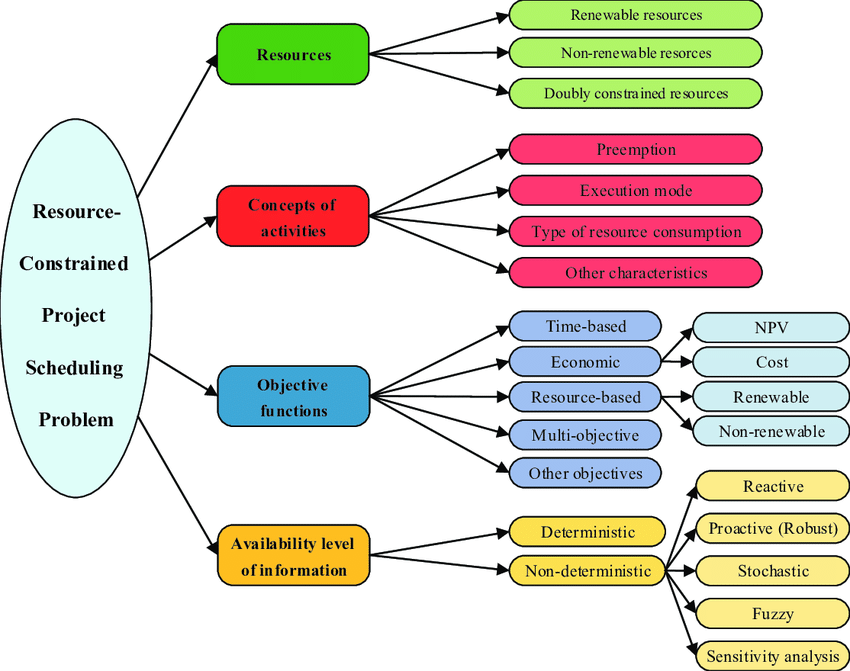
\includegraphics[scale=0.5]{Figures/Classification-of-resource-constrained-project-scheduling-problems.png}
    \caption{Clasificación de RCPSP del artículo: Resource-constrained project scheduling problem: review of past and recent developments (2018)}
    \label{fig:Classification}
\end{figure*}




Y ahora la gran pregunta...
¿RCPSP sirve para otros problemas y aplicaciones reales?

\begin{itemize}
    \item Uso de la energía \textbf{Energy-cost-aware resource-constrained project scheduling for complex product system with activity splitting and recombining (2021)} \cite{du2021energy}. El abstract dice: \textit{"This paper presents a new variant of resource-constrained project scheduling problem (RCPSP), which is named energy-cost-aware resource-constrained project scheduling problem with activity splitting and recombining (eRCPSP-AS\&R) for CoPS"}.
    
    \item Eficiencia energética \textbf{An Optimization of Energy-Efficiency in Machining Manufacturing Systems Based on a Framework of Multi-Mode RCPSP (2016)} \cite{samukawa2016optimization}. El abstract dice: \textit{This paper extends authors’ previous work to a more practical situation to demonstrate the applicability of the proposed framework of energy-efficient manufacturing opera- tions based on a resource-constrained project scheduling problem (RCPSP)}.
    

    \item \textbf{Quantum-Inspired Genetic Algorithm for Resource-Constrained Project-Scheduling (2021)} \cite{saad2021quantum}.

    \item \textbf{Solving the resource constrained project scheduling problem with quantum annealing. 2024.} \cite{perez2024solving}

\item El trabajo \cite{schutt2009cumulative} dice: \textit{Open-Shop-Job problems which is a special case for Rcpsp}. Así lo podemos relacionar con
\textbf{A review of Green shop scheduling problem}  \cite{li2022review},
%\url{https://doi.org/10.1016/j.ins.2021.12.122}
\textbf{A green scheduling algorithm for flexible job shop with energy-saving measures}
\cite{wu2018green},
Subsección 2.3. Energy-efficient scheduling de \textbf{A method for minimizing the energy consumption of machining system: integration of process planning and scheduling} \cite{zhang2016method}

\item Queda por mirar...

\begin{itemize}
    \item Energy-efficient permutation flow shop scheduling problem using a hybrid multi-objective backtracking search algorithm

    \item Dynamic rescheduling in FMS that is simultaneously considering energy consumption and schedule efficiency
\end{itemize}

\end{itemize}


Con restecto a los códigos

\begin{itemize}
    \item Tenemos un listado de los problemas de Minizinc donde está detalladas las funciones que se usa, como por ejemplo \texttt{cumulative}.

\url{https://www.minizinc.org/mznc_list_of_problems_and_globals.html}

    \item El github de Minizinc.

\url{https://github.com/MiniZinc}

    \item Con sus benchmarks

\url{https://github.com/MiniZinc/minizinc-benchmarks}

    \item otra página con muchos ejemplos de minizinc es:

\url{http://www.hakank.org/minizinc/}

    \item MiniZinc Tutorial Files, pues eso... todos los códigos usados en el tutorial de minizinc.

\url{https://people.eng.unimelb.edu.au/pstuckey/COMP90046/resources/models/index.html}

\item Ejemplos tomados por temática (los que usamos en nuestro paper).

\url{https://github.com/MiniZinc/specialization-examples}

\end{itemize}





Por otra parte...
Handbook of Constraint Programming \cite{GlobalConstraints}
(pdf en la carpeta 'papers' del overleaf). Ver:

\begin{itemize}
    \item 22.1 Constraint Programming Models for Scheduling.

    \item 7.2.6 Scheduling with Cumulative Resource Constraints. Definición que nos pueder servir para Cumulative. 

    \item 15.6.4 Cumulative Constraint.

    \item 15.11.3 Example: Planning and Scheduling

\end{itemize}


Una definición del "Flexible job shop scheduling problem está dada en:
A research survey: review of flexible job shop scheduling techniques.
Imran Ali Chaudhry, Abid Ali Khan
First published: 07 August 2015 
\url{https://doi.org/10.1111/itor.12199}.



Deterministic job-shop scheduling: Past, present and future (1999)
\url{https://doi.org/10.1016/S0377-2217(98)00113-1}

A survey of dynamic scheduling in manufacturing systems (2008)
\url{https://doi.org/10.1007/s10951-008-0090-8}. Sonia - No veo nada interesante.

Genetic programming for production scheduling: a survey with a unified framework
\url{https://doi.org/10.1007/s40747-017-0036-x}. Sonia - No veo nada interesante.


The hybrid flow shop scheduling problem
\url{https://doi.org/10.1016/j.ejor.2009.09.024}


Datos de ejecución de jobshop:
\url{https://github.com/hakank/hakank/tree/master/minizinc/jobshop_data}



\section{Empirical Evaluation}
\label{sec:Empirical Evaluation}
In order to evaluate our proposal, the mutation testing technique will be used. At present,
there is no mutation system for Minizinc. Therefore, we have designed and implemented a 
set of mutation operators suitable for MiniZinc, which allowed us to generate mutants to validate the proposal.

\subsection{Mutant operators}
This subsection describes the mutation operators defined for Minizinc. Thirty-nine different mutation operators have been designed and implemented, classified into the following 5 categories according to the nature of the operator to which it is related: relational, logical, arithmetic, quantifier and parameter substitution operators. Each operator, named with capital letters and optionally a number, follows a terminology about the original operator of the MiniZinc program and the operator by which it is replaced, being always of the same category. For instance, 'GE2LT', means that the 'greater than or equal to' operator is replaced by the 'less than' operator. It should be noted that several operators exclusive to the MiniZinc language have been designed and implemented: on the one hand, the category of operators that exchange quantifiers 'forall' for 'exists' (and vice versa); and on the other hand, the parameter substitution operator, named 'CSWAP', which swaps parameters 2 and 3 of the MiniZinc predefined function 'cumulative'.

%\subsection{Mutant generation}

Specifically, faults were seeded applying traditional mutation operators, including arithmetic (AOR), logical(LCR) and relational(ROR)  and parameter-swapping  mutation operators~\cite{PAPADAKIS2019275}. 
%Furthermore, a new MiniZinc-specific mutation operator has been created. It replaces one quantified with another quantified.
Once the mutation system has been implemented with the above set of operators, for the MiniZinc language and the characteristics of the scheduling programs, a set of mutation operators described below have been selected. The application of  operators to several examples of scheduling problems implemented in MiniZinc is shown.

 
\begin{description}
    %\item[MUT$\leq$]
    \item[LE2LT] Changing the relational operator \lstinline|<=|  by  \lstinline|<|.
      The application of this operator appears in the mutant
      \url{https://github.com/LuisLlana/metamorphic_testing_constrints/blob/main/MR%201/basic-MUT-%3C%3D-%3C.mzn}.
    \begin{framed}
\begin{lstlisting}[basicstyle=\ttfamily\fontsize{7}{9}\selectfont]
start[pre[i,1]] + duration[pre[i,1]] <= start[pre[i,2]]
\end{lstlisting}
      \vskip -2em
      \centering$\Updownarrow$
\begin{lstlisting}[basicstyle=\ttfamily\fontsize{7}{9}\selectfont]
start[pre[i,1]] + duration[pre[i,1]] < start[pre[i,2]]
\end{lstlisting}
    \end{framed}
%%% Este es nuevo:
%\item[MUT$\geq$]
\item[LE2GE] Changing the relational operator \lstinline|<=|  by  \lstinline|>=|.
      The application of this operator appears in the mutant
      %\url{https://github.com/LuisLlana/metamorphic_testing_constrints/blob/main/MR%201/basic-MUT-%3C%3D-%3C.mzn}.
    \begin{framed}
\begin{lstlisting}[basicstyle=\ttfamily\fontsize{7}{9}\selectfont]
start[pre[i,1]] + duration[pre[i,1]] <= start[pre[i,2]]
\end{lstlisting}
      \vskip -2em
      \centering$\Updownarrow$
\begin{lstlisting}[basicstyle=\ttfamily\fontsize{7}{9}\selectfont]
start[pre[i,1]] + duration[pre[i,1]] >= start[pre[i,2]]
\end{lstlisting}
    \end{framed}
%% Este también es nuevo:
%\item[MUT$\geq$] 
 \item[LE2EQ]Changing the relational operator \lstinline|<=|  by  \lstinline|==|.
      The application of this operator appears in the mutant
      %\url{https://github.com/LuisLlana/metamorphic_testing_constrints/blob/main/MR%201/basic-MUT-%3C%3D-%3C.mzn}.
    \begin{framed}
\begin{lstlisting}[basicstyle=\ttfamily\fontsize{7}{9}\selectfont]
start[pre[i,1]] + duration[pre[i,1]] <= start[pre[i,2]]
\end{lstlisting}
      \vskip -2em
      \centering$\Updownarrow$
\begin{lstlisting}[basicstyle=\ttfamily\fontsize{7}{9}\selectfont]
start[pre[i,1]] + duration[pre[i,1]] == start[pre[i,2]]
\end{lstlisting}
    \end{framed}
    
%\item[MUT$\forall\exists$] 
  \item[F2E] Changing universal and existential quantifiers.
      The application of this operator appears in the mutant
      \url{https://github.com/LuisLlana/metamorphic_testing_constrints/blob/main/MR%202/basic-MUT-forall-exists.mzn}.
    \begin{framed}
\begin{lstlisting}[basicstyle=\ttfamily\fontsize{7}{9}\selectfont]
constraint exists(i in PREC)
\end{lstlisting}
      \vskip -2em
      \centering$\Updownarrow$
\begin{lstlisting}[basicstyle=\ttfamily\fontsize{7}{9}\selectfont]
constraint forall(i in PREC)
\end{lstlisting}
    \end{framed}

    %\item[MUT$\wedge\vee$]
    \item[D2C]Changing disjunctions by conjunctions. The application of
      this operator appears in the mutant
      \url{https://github.com/LuisLlana/metamorphic_testing_constrints/blob/main/MR%203/jobshopMUT-and-or.mzn}.

    \begin{framed}
\begin{lstlisting}[basicstyle=\ttfamily\fontsize{7}{9}\selectfont]
(s[i,j]+d[i,j]<=s[i,enum_next(TASK,j)]) \/
\end{lstlisting}
      \vskip -2em
      \centering$\Updownarrow$
\begin{lstlisting}[basicstyle=\ttfamily\fontsize{7}{9}\selectfont]
(s[i,j]+d[i,j]<=s[i,enum_next(TASK,j)]) /\
\end{lstlisting}
    \end{framed}
\begin{lstlisting}
\end{lstlisting}

\item[CSWAP$\Leftrightarrow$] Interchanging parameters in function calls. In this case applied to the function "cumulative".
 The application of this operator appear in the mutant
  \url{https://github.com/LuisLlana/metamorphic_testing_constrints/blob/main/MR%204/movingMUThandlers.mzn}.
    \begin{framed}
\begin{lstlisting}[basicstyle=\ttfamily\fontsize{7}{9}\selectfont,
  emph={handlers,duration}, emphstyle={\underbar}]
constraint cumulative(start, handlers, duration, available_handlers);
\end{lstlisting}
      \vskip -2em
      \centering$\Updownarrow$
\begin{lstlisting}[basicstyle=\ttfamily\fontsize{7}{9}\selectfont,
  emph={handlers,duration}, emphstyle={\underbar}]
constraint cumulative(start, duration, handlers, available_handlers);
\end{lstlisting}
    \end{framed}

  \end{description}

\subsection{Mutants generation}
Regarding the mutants generated, the notation mut-MO-N.mzn is followed, where MO indicates the name of the mutation operator applied, and N, the occurrence of this operator in the original minizinc model.

We have generated 77 mutants of the rcpsp.mzn model by applying
the mutation operators described above. \url{ https://github.com/LuisLlana/metamorphic_testing_constrints/tree/main/experiments/benchmarks/Mutants}\\
Such mutants will be run with both the original test suite and the follow-up
tests suite, obtained by the application of the defined  MRs. 


%%% Referencia al survey de Papadakis
% PAPADAKIS2019275

\subsection{Test cases generation}


\newpage
\subsection{Result and Discussion/ Experimental results}

% [!htb]
\begin{table*}[htb]
    \centering
    \begin{tabular}{l|c|c|c}

    j30\_10\_01  &  rcpsp.dzn  & fu-cycle.dzn & fu-all-prec.dzn\\
    makespan  & (original) &  & \\
    \hline
     rcpsp.mzn    & 41 & UNSAT & 157 \\
     (original)   &  &  & \\
     \hline
    
    MUT$\leq$-$<$.mzn & 45 & UNSAT & UNSAT \\
     \hline
    
    MUTforall-exists  & 6 & 0& 6 \\
     \hline
    \end{tabular}
    \caption{rows: codes (mutations); columns: data (follow-ups). UNSAT is the sort-name of UNSATISFIABLE }
    \label{tab:outs}
\end{table*}

En la tabla \ref{tab:outs} hay que comparar:
\begin{itemize}
    \item MR1: Si se ponen todas las precedencias en secuencial (fu-all-prec.dzn) entonces el makespan (157) debe ser finito y mayor o igual al original rcpsp.dzn (41). Esto es lo que ocurre al ejecutar el código original (rcpsp.mzn).

    El mutante MUT$\leq$-$<$.mzn se puede matar porque no es finito.

    El mutante MUTforall-exists no se puede matar.

    \item MR2: Si se crea un ciclo con las precedencias (fu-cycle.dzn), entonces debe ser UNSATISFIABLE. Esto es lo que ocurre al ejecutar el código original (rcpsp.mzn).

    El mutante MUT$\leq$-$<$.mzn no se puede matar.

    El mutante MUTforall-exists se puede matar pues tiene un resultado finito (0).

\end{itemize}

\newpage
\newpage

%En la ayuda de un error de overleaf me ha dicho: \textit{Pretend that you're Hercule Poirot: Examine all clues, and deduce the truth by order and method.}

%Es decir, \textit{Imagina que eres Hércules Poirot: examina todas las pistas,
% y deducir la verdad por orden y método.}





%\input{Sections/...}




 \bibliographystyle{elsarticle-num}
 \bibliography{biblio}


\end{document}

%%% Local Variables:
%%% mode: latex
%%% TeX-master: t
%%% End:


